% THIS IS SIGPROC-SP.TEX - VERSION 3.1
% WORKS WITH V3.2SP OF ACM_PROC_ARTICLE-SP.CLS
% APRIL 2009
%
% It is an example file showing how to use the 'acm_proc_article-sp.cls' V3.2SP
% LaTeX2e document class file for Conference Proceedings submissions.
% ----------------------------------------------------------------------------------------------------------------
% This .tex file (and associated .cls V3.2SP) *DOES NOT* produce:
%       1) The Permission Statement
%       2) The Conference (location) Info information
%       3) The Copyright Line with ACM data
%       4) Page numbering
% ---------------------------------------------------------------------------------------------------------------
% It is an example which *does* use the .bib file (from which the .bbl file
% is produced).
% REMEMBER HOWEVER: After having produced the .bbl file,
% and prior to final submission,
% you need to 'insert'  your .bbl file into your source .tex file so as to provide
% ONE 'self-contained' source file.
%
% Questions regarding SIGS should be sent to
% Adrienne Griscti ---> griscti@acm.org
%
% Questions/suggestions regarding the guidelines, .tex and .cls files, etc. to
% Gerald Murray ---> murray@hq.acm.org
%
% For tracking purposes - this is V3.1SP - APRIL 2009

\documentclass{acm_proc_article-sp}

\usepackage{graphicx}
\usepackage{subfigure}

\begin{document}

\title{Better JavaScript Runtime Understanding by Automated Function Name Extraction}
%
% You need the command \numberofauthors to handle the 'placement
% and alignment' of the authors beneath the title.
%
% For aesthetic reasons, we recommend 'three authors at a time'
% i.e. three 'name/affiliation blocks' be placed beneath the title.
%
% NOTE: You are NOT restricted in how many 'rows' of
% "name/affiliations" may appear. We just ask that you restrict
% the number of 'columns' to three.
%
% Because of the available 'opening page real-estate'
% we ask you to refrain from putting more than six authors
% (two rows with three columns) beneath the article title.
% More than six makes the first-page appear very cluttered indeed.
%
% Use the \alignauthor commands to handle the names
% and affiliations for an 'aesthetic maximum' of six authors.
% Add names, affiliations, addresses for
% the seventh etc. author(s) as the argument for the
% \additionalauthors command.
% These 'additional authors' will be output/set for you
% without further effort on your part as the last section in
% the body of your article BEFORE References or any Appendices.

\numberofauthors{3} %  in this sample file, there are a *total*
% of EIGHT authors. SIX appear on the 'first-page' (for formatting
% reasons) and the remaining two appear in the \additionalauthors section.
%
\author{
% You can go ahead and credit any number of authors here,
% e.g. one 'row of three' or two rows (consisting of one row of three
% and a second row of one, two or three).
%
% The command \alignauthor (no curly braces needed) should
% precede each author name, affiliation/snail-mail address and
% e-mail address. Additionally, tag each line of
% affiliation/address with \affaddr, and tag the
% e-mail address with \email.
%
% 1st. author
\alignauthor
Salman Mirghasemi\\
       \affaddr{\'Ecole Polytechnique F\'ed\'erale de Lausanne}\\
       \affaddr{Lausanne, Switzerland}\\
       \email{salman.mirghasemi@epfl.ch}
% 2nd. author
\alignauthor
John J. Barton\\
       \affaddr{IBM Research - Almaden}\\
       \affaddr{San Jose, USA}\\
       \email{johnjbarton@johnjbarton.com}
% 3rd. author
\alignauthor Claude Petitpierre\\
       \affaddr{\'Ecole Polytechnique F\'ed\'erale de Lausanne}\\
       \affaddr{Lausanne, Switzerland}\\
       \email{claude.petitpierre@epfl.ch}
}


\maketitle
\begin{abstract}
Understanding JavaScript code due to its dynamic, weakly-typed nature is complicated. Developers usually understand JavaScript programs by running them and examining their elements at runtime. However, understanding concrete values, particularly user-defined and function objects, is not always straightforward. Function names can aid in this regard; they can appear as the constructor name in object representation or as the functions identifier in callstack. Unfortunately, only a very low proportion (less than 10\%) of JavaScript functions are named by developers in the first place. As a solution to this issue, we propose an approach for automated JavaScript function naming based on source code analysis. We applied our approach on several JavaScript projects and the resutls are very promising.

\end{abstract}

\category{D.2.5}{Testing and Debugging}{Debugging aids}
\category{D.2.6}{Programming Environments}{Integrated environments}

\terms{Algorithms, Human Factors, Languages}

\keywords{Debugging, JavaScript, Function Name} % NOT required for Proceedings

\section{Introduction}
The unique and important role of JavaScript in web programming is undeniable. Along with the wave of ``Web 2.0", JavaScript has become the inevitable part of almost every modern web site. This language is used by 97 out of the web's 100 most popular sites\footnote[1]{http://www.alexa.com}. It is very likely that JavaScript keeps this crucial role at least for the next few years. Along with the growth of demands for more comprehensive user interfaces, the size and the complexity of web applications is increasing. Morover, JavaScript is also becoming a general purpose computing platform with office applications \cite{JSOffice, JSOffice2}, browsers \cite{FAO, GCE} and development environments \cite{Ingalls} being developed in JavaScript \cite{Richards}. There are also proposals for employing JavaScript in server-side applications \cite{SSJSR, CJS}.


\begin{figure*}[htp]
\centerline{
\subfigure[Google Chrome Debugger]{\label{fig_object_second_case}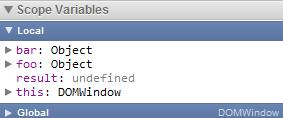
\includegraphics[width=0.47\textwidth,height=.15\textheight]{pic/chrome-objects.jpg}}
\hfil
\subfigure[Firebug]{\label{fig_object_first_case}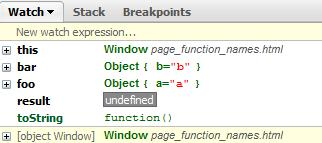
\includegraphics[width=.47\textwidth,height=.15\textheight]{pic/fbug-objects.jpg}}}
\caption{The screenshot of veriables view of Google Chrome and Firebug JavaScript debuggers displaying the same program state.}
\label{debuggers-objects}
\end{figure*}


To cope with the pace of changes, JavaScript developers need to improve their develoment processes and practices. They need modern editors for writing and editing larger programs and effective tools for understanding complicated JavaScript runtime. However, there has been severe inherent barriers for improving JavaScript tool support. 
JavaScript, unlike many traditional object oriented languages such as Java and C\#, does not have classes, and does not encourage encapsulation or even structured programming. JavaScript is a weakly typed language with no type declarations and only run-time checking of calls and field accesses \cite{Richards}. As a direct consequence, the JavaScript code contains less explanatory data about the program elements and their relations. The value of a variable can be a primitive value, an object with any structure or even a function. One callsite may invoke different function bodies with different number of arities that none of them can be understood from the code. Therefore, the lack of descriptive data in JavaScript code is the most fundumental issue in enhancing JavaScript tool support.

Catching errors early (i.e., before or at the compilation time) is an important feature for development environments. It can save developers' time, prevent bugs and improve the program reliability. However, many errors can not be recognized without a strong typing stystem. To attack this issue a few static typing systems have been proposed for JavaScript \cite{Anderson, Anderson2, Heidegger, Thiemann}. These approaches discover the type of values and object structures for a variable by statically analyzing the source code and possible program control flows lead to the variable assignment. These discovered facts about variable types are not only useful for catching errors but to provide modern editing features such as auto-complete and refactoring in development environments. Moreover, these infered data can help in code coprehension if they are properly presented. Nevertheless, none of the mentioned approaches provided effective means for sharing this information with the developer. 

Developers usually understand JavaScript code by examining the running program in debuggers. At runtime, concrete values are available and the developer can directly check and understand object structures and control flows. Understanding a concrete value, particulary for non-primitive values such as objects and functions, is not always straightforward. To facilitate understanding these complex values at the first place, debuggers show a summary of these objects. For example, in case of user-defined objects, the name of object's constructor can be very helpful in the object summary. It can work like a class name and summarizes the object structure.

Functions are central to program comprehension in JavaScript. They are first-class objects that are used for different purposes by developers; 
they may be used as an object  constructor, a clousure scope(module) or even  passed as an argument in a function call. However, there is a subtle issue with JavaScript functions that makes working with them quite difficult: functions can be defined and created with no name or identifier. This problem particularly shows up in debuggers \cite{Zaytsev}. The function name is necessary for referring and recalling the function's functionality, but only a small proportion (less than 10\%) of JavaScript functions are named.

In this paper, we propose automated JavaScript function naming based on extracted data from the source code. The candidate function names can be used in debuggers for more descriptive object summaries and callstack view. Moreover, these function names can be used in integration with proposed JavaScript typing systems for providing modern editing features in development environments.

\begin{figure*}[htp]
\centerline{
\subfigure[Google Chrome Debugger]{\label{fig_second_case}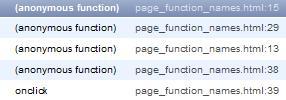
\includegraphics[width=0.47\textwidth,height=.13\textheight]{pic/chrome-callstack.jpg}}
\hfil
\subfigure[Firebug]{\label{fig_first_case}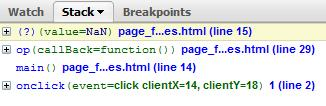
\includegraphics[width=.47\textwidth,height=.13\textheight]{pic/fbug-callstack.jpg}}}
\caption{The screenshot of callstack view of Google Chrome and Firebug JavaScript debuggers paused at the same breakpoint.}
\label{debuggers-callstack}
\end{figure*}

\section{The Function Naming Problem}

A JavaScript function can be defined in different ways: by the {\small\texttt{function}} operator (i.e., function decleration or expression) or the {\small\texttt{Function}} constructor (i.e., {\small\texttt{new Function(args, source)}}) \cite{ECMA}. Once a statement which defines a function is evaluated, a {\small\texttt{Function}} object is created. Notice that, depending on the times a function definition is evaluated, zero to many {\small\texttt{Function}} objects can be created from that definition. To classify {\small\texttt{Function}} objects created by the same code, we call every script defines a function as a \textit{function body}. 

{\small\texttt{Function}} objects have no name by default; as the {\small\texttt{Function}} constructor doesn't receive any name. According to ECMA specification, a function name (identifier) can be specified after the {\small\texttt{function}} operator (It is mandatory for function declerations but optional for function expressions) \cite{ECMA}. However, the usage of function identifiers is limited. The reason is that, function names, in addition to naming the function, has an effect on available variables in the scopes. In the case of function declearations, the function object is assigned to a variable in the function scope, but in the case of function expressions, the function object is available only inside the function. The confusing behavior of function identifiers get worse by function statements introduced by some browser such as Firfox. Function statements are like function expressions, but the function object is available in the entire function scope like function declarations \cite{Zaytsev}. Therefore, developers often prefer to omit the function identifier in the function statement to avoid its confusing impact.

Functions in JavaScript are first-class objects. They can be assigned to any variable or object proeprty, or passed as an argument to a function. It is common that the same function is called by various names in different contexts. Therefore, it is usually very difficult to recall the function operation from its local name. Developers have usually the option to look at the function code, but it is tedious and time-consuming. Two main issues apears in debuggers due to the lack of function name. First, object constructor name which can faciliate understanding the object value, is not available in the object summary. Second, the callstack view is usually full of \textit{anonymous} functions and therefore less informative. We disscuss these issues in the next two subsections.
 
\subsection{Constructor Name}
JavaScript doesn't support classes, but objects can be created by constructors ({\small\texttt{new Constructor()}}). A constructor is a regular JavaScript function. Once the {\small\texttt{new}} keyword is evaluated, an empty object, with the constructor prototype as its prototype, is created, then the new object is bound to {\small\texttt{this}} and the constructor is called. The role of constructor is to initialize the empty object. Although the structure of object imposed by the constructor, unlike class-based object-oriented languages, may not remain intact during the object's lifetime \cite{Richards}, the constructor can still be used to classify the object. 
Debuggers employ this fact and display the constructor name in the object summary to facilitate developer's understanding. 

Figure~\ref{js-code} demonstrates an excerpt of a JavaScript code. We set a breakpoint on line 13 and examin the runtime elements at this breakpoint by two JavaScript debuggers, Google Chrome and Firebug (Figure~\ref{debuggers-objects}). Two objects assigned to variables {\small\texttt{foo}} and {\small\texttt{bar}} are constructed by two different constructors: {\small\texttt{FOO}} and {\small\texttt{BAR}}. However, Google Chrome debugger shows the general class of {\small\texttt{Object}} as the summary for both objects. The developer has to expand the object nodes to recognize their similarities and differences. Firebug classify objects in the same general class, but includes some of the object properties in the summary. These additional properties may hint develooper about the object structures. {\small\texttt{FOO}} and {\small\texttt{BAR}} definitions at lines 19 and 22 explain this behaviour; the function statements has no explicit name (identifier), therefore debuggers considered them as \textit{anonymous} functions.


\begin{figure}[htp]
{\small 
\begin{verbatim}
9  var main = function(){
10   return function(){
11     var foo = new FOO("a");
12     var bar = new BAR("b");
13     var result = op(
14       function(value){
15         return value;
16        });
17   }
18 }();
19 var FOO = function(a){
20   this.a = a;
21 }
22 var BAR = function(b){
23   this.b = b;
24 }
25 var op = function(){
26   var local;
27   return function(callBack){
28     local++;
29     return callBack(local);
30   }
31 }();
\end{verbatim}}
\caption{An excerpt of a JavaScript code.}
\label{js-code}
\end{figure}

\subsection{Callstack View}
To illustrate the second issue, we pause the program (Figure~\ref{js-code}) at line 15 by a breakpoint. Figure~\ref{debuggers-callstack} shows how the program callstack is displayed in Google Chrome debuggers and Firebug. The differences in the number of frames and line numbers between two callstacks are due to dissimilar event handling implementations in the underlying platforms. Google chrome shows {\small\texttt{anonymouse}} as the name of all functions excepting the first one. Firebug performs better by guessing three function names but it still fails in one case. In these cases, the information provided by debugger is useless and the developer has to locate the function source to understand or recall the function behaviour. 

The other pieces of information which are important at function calls are {\small\texttt{this}} and argument values. In JavaScript, {\small\texttt{this}} like arguments is not defined by lexical scopes but it is bound once the function is called. The {\small\texttt{this}} value is missed in both views. The arguments values is shown in Firebug, but it still sufferes from similar issues explained for displaying object summaries.

\section{Automated Funcation Naming}
    To tackle the aforementioned function naming issues, we propose automated function naming by anlysing the source code. A function name must help the developer to
distinguish the function from other functions with different behaviours. The behaviour of a function is dependent to its source code, enclosing scopes (because of global and closure variables), the object bound to {\small\texttt{this}}-depending how it is called- and passed arguments. The first two parameters can be almost known from the source code, while the two last parameters are usually not known until the function call at runtime. Therefore, to name a function object, it is enough to name its \textit{function body}. 
    A function body can be uniquly identified by its location in the source file. A naive proposal for the function name for a function body is a combination of the function file name and line number. Although it may work as an identifier, but it does not assist the develper to recall or understand the function behaviour. 
    
In contrast, we use names in the source code to name nameless functions. 
    Once a function object is created, one of these cases would happen:
    \begin{enumerate}
		\item the function object is assigned to a variable or one of its properties.
		\item it is assigned to a property of a new object.
		\item it is assigned to a new array index.
		\item it is called.
		\item it is returned from a function call.
		\item it is passed as an argument to a function.
		\end{enumerate}
   

To choose the most appropriate name for a function which has the characteristics defined in the previous section, we consider two cases. First, assigning a global name to the function which identifies the function in the whole program. Second, naming a function in a call stack.

A function object in JavaScript can be defined by \texttt{function \textit{identifier} (args)\{...\}} or \texttt{new Function(args, source)}.
\subsection{A Global Name for a Function Object}


%\begin{center}
    %\begin{tabular}{ | l | l | l | p{5cm} |}
    %\hline
    %& Type & Sample & Description \\ \hline
    %a & Named & function foo(){...} & The function is named. \\ \hline
    %a & Named & function foo(){...} & The function is named. \\ \hline
    %a & Named & function foo(){...} & The function is named. \\ 
    %\hline
    %\end{tabular}
%\end{center}


\begin{figure}[htp]
\begin{verbatim}
(a) Case 1:
 function foo(){ ... }

(b) Case 2:
 var foo = function { ... } 
 
(c) Case 3:
 var foo = {
     bar : function { ...}
 }

(d) Case 4:

 var foo = function(){
           ....
           return function(){ ... }
 }()
 
(e) Case 5:
 var foo = function(){ 
 					 return ...;
 }()					
 
(f) Case 6:
 var foo = function(){
 
 }()();
 
(g)
 foo(function(){ ... });
 
(h)
 array = [...., function(){},...]
 
(i)
 array[i] = function(){};   

(j)
 eval(); & new Function("");
 
\end{verbatim}
\caption{Different cases of function object creation.}
\label{fig:functionCreation}
\end{figure}

\subsection{Naming Functions in Call Stack}
%new Function ([arg1[, arg2[, ... argN]],] functionBody)
%this[ optall.queue === false ? "each" : "queue" ](function() {})

%The object referenced by the keyword {\small\texttt{this}} is not determined by lexical scoping, but instead by the caller;
\begin{figure}[htp]
\begin{verbatim}
(a)
 foo();
(b)
 foo.bar();
(c)
 foo.apply(bar, args);
(d)
 foo.call();
\end{verbatim}
\caption{Different cases of function object creation.}
\label{fig:functionCall}
\end{figure}

\section{evaluation}
%Firebug, JQuery,

%JQuery
% core.js 

%namespaces in JS:http://javascriptweblog.wordpress.com/2010/12/07/namespacing-in-javascript/
%commonjs requriejs, ...
%the function name not very long like google chrome  xxxx.yyy.zzz

\section{Related Work}










\section{Conclusion}
In this paper we presented an approach for naming JavaScript functions both
as individual objects and in call stack. 


%ACKNOWLEDGMENTS are optional
%\section{Acknowledgments}

%
% The following two commands are all you need in the
% initial runs of your .tex file to
% produce the bibliography for the citations in your paper.

%\bibliographystyle{abbrv}
%\bibliography{sigproc}  % sigproc.bib is the name of the Bibliography in this case
% You must have a proper ".bib" file
%  and remember to run:
% latex bibtex latex latex
% to resolve all references
%
% ACM needs 'a single self-contained file'!
%
%APPENDICES are optional
%\balancecolumns

\begin{thebibliography}{10}

\bibitem{Anderson}
C. Anderson, P. Giannini, and S. Drossopoulou. \newblock Towards Type Inference for JavaScript.
\newblock In \emph{Proceedings of the 19th European conference on Object-Oriented Programming(ECOOP)},
July, 2005.

\bibitem{Anderson2}
C. Anderson and P. Giannini. \newblock Type checking for javascript.
\newblock \emph{Electr. Notes Theor. Comput. Sci.}, 138(2), 2005. 

\bibitem{CJS}
Common JS.
\newblock http://www.commonjs.org/

\bibitem{ECMA}
ECMA International.
\newblock \emph{ECMA-262: ECMAScript Language Specification},
ECMA (European Association for Standardizing Information
and Communication Systems), Geneva, Switzerland, third edition,
December 1999. 

\bibitem{FAO}
Firefox Add-ons.
\newblock https://addons.mozilla.org/en-US/developers/docs/gett ing-started.

\bibitem{GCE}
Google Chrome Extensions.
\newblock http://code.google.com/chrome/extensions.

\bibitem{Heidegger}
P. Heidegger and P. Thiemann.\newblock Recency types for dynamically-typed, object-based languages.
\newblock In \emph{Proceedings of Foundations of Object Oriented Languages (FOOL)},
2009.

\bibitem{Ingalls}
D. Ingalls, K. Palacz, S. Uhler and A. Taivalsaari.\newblock The lively kernel a self-supporting system on
a web page.
\newblock In \emph{Self-Sustaining Systems},
2008.

\bibitem{JSOffice}
JScript development in Microsoft Office 11.
\newblock http://msdn.microsoft.com/ en-us/library/aa202668(office.11).aspx

\bibitem{JSOffice2}
JavaScript development in OpenOffice.
\newblock http://framework.openoffice.org/ scripting/release-0.2/javascript-devguide.html

\bibitem{Richards}
G. Richards, S. Lebresne, B. Burg and J. Vitek.\newblock An analysis of the dynamic behavior of JavaScript programs.
\newblock In \emph{Proceedings of the 2010 ACM SIGPLAN conference on Programming language design and implementation(PLDI)},
June, 2010.

\bibitem{SSJSR}
Server-Side JavaScript Reference v1.2.
\newblock http://research.nihonsoft.org/ javascript/ServerReferenceJS12.

\bibitem{Thiemann}
P. Thiemann.\newblock Towards a type system for analyzing JavaScript programs.
\newblock In \emph{Proceedings of European Symposium on Programming (ESOP)},
2005.

\bibitem{Zaytsev}
J. Zaytsev.\newblock Named function expressions demystified.
\newblock http://kangax.github.com/nfe,
June, 2010.


\end{thebibliography}



\end{document}
